%%%%%%%%%%%%%%%%%%%%%%%%%%%%%%%%%%%%%%%%%%%%%%%%%%%%%%%%%%%%%%%%%%%%%%%%

%%% LaTeX Template for AAMAS-2021 (based on sample-sigconf.tex)
%%% Prepared by Natasha Alechina and Ulle Endriss (version 2020-08-06)

%%%%%%%%%%%%%%%%%%%%%%%%%%%%%%%%%%%%%%%%%%%%%%%%%%%%%%%%%%%%%%%%%%%%%%%%

%%% Start your document with the \documentclass command.
%%% Use the first variant below for the final paper.
%%% Use the second variant below for submission.

% \documentclass[sigconf]{aamas} 
\documentclass[sigconf,anonymous]{aamas} 


%%% Load required packages here (note that many are included already).
\usepackage{soul}
\usepackage{subcaption}
\usepackage[export]{adjustbox}


%%%%%%%%%%%%%%%%%%%%%%%%%%%   MACROS   %%%%%%%%%%%%%%%%%%%%%%%%%%%%%%%%%

\newcommand{\xmu}[2]{x_{#1_#2}^{#2}(t)}
\newcommand{\xmudash}[2]{x_{#1_#2}^{#2}(t')}
\newcommand{\payoff}[2]{P^{#2}_{#1_#2, #1_{-#2}}}

\newcommand{\dxmu}[1]{\dot{x}_{#1_\mu}^{\mu} (t)}
\newcommand{\hxmu}[1]{\hat{x}_{#1_\mu}^{\mu} (t)}
\newcommand{\hxnu}[1]{\hat{x}_{#1_\nu}^{\nu} (t)}
\newcommand{\hxmudash}[1]{\hat{x}_{#1_\mu}^{\mu} (t')}
\newcommand{\hxnudash}[1]{\hat{x}_{#1_\nu}^{\nu} (t')}

\newcommand{\txmu}[2]{\tilde{x}_{#1_#2}^{#2}(t)}
\newcommand{\dtxmu}[2]{\dot{\tilde{x}}_{#1_#2}^{#2}(t)}
\newcommand{\tpayoff}[2]{\tilde{P}^{#2}_{#1_#2, #1_{-#2}}}
\newcommand{\talpha}{\tilde{\alpha}}
\newcommand{\ttau}{\tilde{\tau}}
\newcommand{\htau}{\hat{\tau}}
\newcommand{\xfixed}{x_\infty}
\newcommand{\ezerof}{\eta_{0, \infty}}
\newcommand{\eonef}{\eta_{1, \infty}}

\newcommand{\xpert}{\hat{x}(t)}
\newcommand{\xpertdash}{\hat{x}(t')}
\newcommand{\ezeropert}{\hat{\eta}_0(t)}
\newcommand{\eonepert}{\hat{\eta}_1(t)}

\newcommand{\eom}{\frac{\dxmu{i}}{\xmu{i}{\mu}} - \alpha \ttau \left ( \sum_{i_{-\mu}} \payoff{i}{\mu} \prod_{\kappa \neq \mu} \xmu{i}{\kappa} \right ) + \\ \alpha \htau \left ( \frac{1}{\sqrt{N}} \sum_{i_\mu i_{-\mu}} \xmu{i}{\mu} \payoff{i}{\mu} \prod_{\kappa \neq \mu} \xmu{i}{\kappa} \right ) - \talpha \rho^{\mu}_{i}(t)}

\usepackage{xcolor} % REMOVE THIS AT THE END
\newcommand\fb[1]{\textcolor{blue}{FB: #1}}
\newcommand\ah[1]{\textcolor{red}{AH: #1}}
%%%%%%%%%%%%%%%%%%%%%%%%%%%%%%%%%%%%%%%%%%%%%%%%%%%%%%%%%%%%%%%%%%%%%%%%

%%% AAMAS-2021 copyright block (do not change!)

\setcopyright{ifaamas}
\acmConference[AAMAS '21]{Proc.\@ of the 20th International Conference on Autonomous Agents and Multiagent Systems (AAMAS 2021)}{May 3--7, 2021}{London, UK}{U.~Endriss, A.~Now\'{e}, F.~Dignum, A.~Lomuscio (eds.)}
\copyrightyear{2021}
\acmYear{2021}
\acmDOI{}
\acmPrice{}
\acmISBN{}

%%%%%%%%%%%%%%%%%%%%%%%%%%%%%%%%%%%%%%%%%%%%%%%%%%%%%%%%%%%%%%%%%%%%%%%%

%%% Use this command to specify your EasyChair submission number.
%%% In anonymous mode, it will be printed on the first page.

\acmSubmissionID{489}

%%% Use this command to specify the title of your paper.

\title[InstabilityinMARL]{Stability and Chaos in Multi-agent Reinforcement Learning}

%%% Provide names, affiliations, and email addresses for all authors.

\author{Aamal Hussain}
\affiliation{
  \department{Department of Computing}
  \institution{Imperial College London}}
\email{aamal.hussain15@imperial.ac.uk}

\author{Francesco Belardinelli}
\affiliation{
  \department{Department of Computing}
  \institution{Imperial College London}}
\email{francesco.belardinelli@imperial.ac.uk}


%%% Use this environment to specify a short abstract for your paper.

\begin{abstract}
Modelling the dynamics of Q-Learning is an active and important topic
for the sake of developing an {\em a priori} understanding of
Reinforcement Learning. In this paper, we use methods from
evolutionary game theory to analyse the stability of Q-Learning in
$p$-player games, where payoffs are randomly generated. We determine
the parameter range in which Q-Learning is expected to settle to a
stable fixed point and the range in which the dynamics are unstable.

This study allows for parameters to be appropriately chosen to ensure
the safe convergence of a learning algorithm and as a first step
towards understanding the range of behaviours that can be displayed by
learning using the Q-Learning algorithm. We validate our theoretical
results through numerical simulation and show that, within the bounds
of experimental error, the region of instability can be characterised
by the learning dynamics.
\end{abstract}

%%% The code below was generated by the tool at http://dl.acm.org/ccs.cfm.
%%% Please replace this example with code appropriate for your own paper.


%%% Use this command to specify a few keywords describing your work.
%%% Keywords should be separated by commas.

\keywords{Reinforcement Learning, Dynamical Systems, Game Theory.}

%%%%%%%%%%%%%%%%%%%%%%%%%%%%%%%%%%%%%%%%%%%%%%%%%%%%%%%%%%%%%%%%%%%%%%%%

%%% Include any author-defined commands here.
         
\newcommand{\BibTeX}{\rm B\kern-.05em{\sc i\kern-.025em b}\kern-.08em\TeX}

%%%%%%%%%%%%%%%%%%%%%%%%%%%%%%%%%%%%%%%%%%%%%%%%%%%%%%%%%%%%%%%%%%%%%%%%

\begin{document}

%%% The following commands remove the headers in your paper. For final 
%%% papers, these will be inserted during the pagination process.

\pagestyle{fancy}
\fancyhead{}

%%% The next command prints the information defined in the preamble.

\maketitle 

%%%%%%%%%%%%%%%%%%%%%%%%%%%%%%%%%%%%%%%%%%%%%%%%%%%%%%%%%%%%%%%%%%%%%%%%

\section{Introduction}
\label{sec::Intro}

Single agent reinforcement learning (RL) is a well-established
framework for allowing agents to learn optimal strategies when trained
on an iterated task
%For a particularly strong example of this see
\cite{Vinyals2019}. However, for the realisation of complex tasks,
such as air traffic control, market negotiations, and multi-robot
coordination, it is required that the system be modelled as a
multi-agent system (MAS). Such systems are not as well-understood as
single-agent systems in RL, since a given agent is tasked with
optimising a reward function which depends not only on a
non-stationary environment, but also on the actions of other, possibly
loosely coupled, agents \cite{SchwartzMulti-agentApproach}.

It is, therefore, of paramount importance to develop a strong
theoretical understanding of multi-agent reinforcement learning (MARL)
to allow an {\em a priori} understanding of the behaviour of a given
learning algorithm. Fortunately, the study of MAS is not unique to the
field of AI and has been extensively investigated from the point of view of
economics and game theory as well
\cite{ShohamMultiagentFoundations}. In particular,
%the study of
evolutionary game theory (EGT) considers the problem of a MAS which is
repeatedly exposed to an iterated game. This idea shares a strong
resemblance with MARL and, in fact, in \cite{Tuyls2006AnGames} it was
shown that techniques from EGT may be fruitfully applied to the analysis of
Q-Learning \cite{Sutton2018}.

An important result in modelling such multi-agent systems from the EGT
perspective is that, when games are learnt and the assumptions of
rationality and perfect information are lifted, games may not converge
to an equilibrium. Instead, as shown in \cite{Sanders2018}, the
dynamics may be more complex, and even chaotic (see
Sec.~\ref{sec::DynamicalBehaviours}). The present work further
describes that the emergence of such behaviours depends on the
parameters of the games and the learning algorithm. For the analysis
of multi-agent systems whose behaviour is inter-dependent, it is
desirable that the system be such that the game converges to a
stable equilibrium. Without this, it is inherently impossible to
predict the outcome of learning.

\paragraph{Contribution}
In this study, we will be considering the question: under what choice
of parameters is a multi-agent system, which is trained on an iterated normal-form game using Q-Learning, likely to converge to an equilibrium as opposed
to displaying complex, or unstable behaviours? In investigating this
question, we will make the following assumptions:

\begin{enumerate}
    \item There is a finite set of agents, though its size $p$ can be
      arbitrarily large.
      
    \item The agents have a large, but discrete, strategy space:
      during the theoretical study, we will make the assumption that
      the number $N$ of actions goes to infinity.

  \item The agents are homogeneous. This requires that all agents have
    the same parameters and are trained using the same
    algorithm. Since this is typically the case in reinforcement
    learning studies, it is not an unreasonable assumption, but does
    present an interesting avenue for future work.

  \item The agents are trained on stateless, normal form games
    (i.e., the environment is static).
\end{enumerate}

Through our analysis and experiments we find that likelihood of
displaying unstable dynamics increases as the \textit{step length}
$\alpha$ and \textit{intensity of choice} $\tau$ parameters in the
Q-Learning algorithm
%\cite{Barber2012}
increase. However, the
correlation $\Gamma$ between payoffs, which measures how cooperative
or competitive a game is, does not affect the stability of the
system. In addition, we find that regardless of the choice of these
parameters, the likelihood of unstable behaviours increases as the
number  $p$ of players in the game increases.

\subsection*{Related Work}

In this section we present an overview of the vast literature which
considers the study of reinforcement learning from an evolutionary
game dynamics perspective, as well as touching upon some important
results and research within the field of game dynamics.

\paragraph{Evolutionary Game Dynamics}
The theory of evolutionary game dynamics \cite{Morgenstern44}
considers game-like settings in which agents must repeatedly interact
with one another. The outcome of this interaction depends on a payoff
matrix; 'strong' strategies which maximise the reward are promoted,
whilst 'weaker' strategies diminish. The \textit{replicator dynamic}
models this behaviour, and allows one to determine whether, after a
number of iterations, the game is likely to converge to some fixed
equilibrium and, if so, the probabilities with which strategies are
played in this equilibrium \cite{ShohamMultiagentFoundations}.
%for an excellent introduction to the replicator dynamics).

Analyses have been performed from the perspective of the replicator
dynamic w.r.t.~the various types of behaviours that can emerge from
iterated games. Such games are considered imperfect, in that agents
make decisions by attempting to anticipate their opponents' behaviour
based on experience \cite{Galla2011}. \cite{Imhof2005} presents the
observation that, in the Prisoner's Dilemma, cyclic behaviour
emerges in which the optimal strategy cycles across defection,
cooperation and tit-for-tat despite defection being the
NE. In \cite{Galla2011}, Galla builds on this observation by showing that, in fact,
such behaviour is highly dependent on the presence of memory loss in
the system. In the absence of memory loss, the learning converges to
the NE as expected.
%However, as this parameter is increased, the stability of the NE is
%removed and other stable points are created.

Taking the notion of parameter dependence further, \cite{Galla2013}
describes an analysis of two-player iterated games in which the
players learn using \textit{experience weighted attraction} (EWA), a
form of reinforcement learning typically applied in experimental
economics \cite{Camerer2009}. Through numerical simulations, the
authors are able to show that the emergence of chaos and cycles is
dependent on the choice of parameters.
%(see \cite{Strogatz2000} for
%details on chaotic and periodic motion).
A rigorous theoretical analysis of the replicator dynamic
corresponding to EWA, which applies the techniques in
\cite{Opper1992}, results in a method for characterising the regions
in parameter space in which a game is likely to converge, exhibit
chaos or limit cycles. More recently, the same authors presented an
extended study in \cite{Sanders2018}, in which the same analysis is
applied to generic $p$-player games, which showed that chaotic
dynamics are more likely to be observed as the number $p$ of players
increases. Differently from this line, we here consider 
%By contrast to the present work, \cite{Barber2012} focuses
%on the analysis of the EWA algorithm, while we consider
 Q-Learning \cite{Barber2012}, which is one of the most popular
 algorithms in RL.

It is evident, therefore, that in the case of learning on iterated
games, convergence to stable equilibria cannot be taken for granted
and, in fact, is rare. It would therefore be fruitful to bring these
analyses from EGT to better understand reinforcement learning from an
AI perspective.

\paragraph{Dynamics of RL}
In \cite{Tuyls2006AnGames}, the authors are able to derive a relation
between Q-Learning
%(see \cite{Barber2012})
and the replicator
dynamic. In doing so, the authors present an evolutionary model which
accurately predicts the dynamics of Q-Learning. This sprung forward a
vast array of literature which performs similar derivations for various
RL algorithms \cite{Bloembergen2015}.
%for an
%excellent literature review).
In particular,
%it should be noted that
many of these studies focus on normal form games, in which the payoff
matrix does not change (i.e., the environment is static). Recent work,
such as \cite{Hennes2008}, extends this framework towards multi-state
games.
%though this is restricted to 2 state games.
Similarly, \cite{Galstyan2013} extends the work in
\cite{Tuyls2006AnGames} towards games with continuous action
spaces. More recently, \cite{Hu2019} considers Q-learning in the
mean-field limit, in which the strategies of populations of agents are
considered, rather than individuals.

The relation between reinforcement learning and the replicator dynamic
allows for the assumption of convergence in RL to be lifted and
instead for the emergence of more complex behaviours to be
examined. In particular, this study aims to perform an analysis
similarly to \cite{Sanders2018} and establish the regions in parameter
space in which Q-Learning converges to stable fixed points.
%and where the learning is unstable.
In doing so, we extend the dynamics considered by Tuyls et al.~to
a general $p$-player setting, rather than two players only, thereby
allowing an analysis of how the number of players in a game affects
its stability.

%%%%%%%%%%%%%%%%%%%%%%%%%%%%%%%%%%%%%%%%%%%%%%%%%%%%%%%%%%%%%%%%%%%%%%%%

\section{Preliminaries}

In this section we establish some of the preliminaries which
are required to follow the subsequent sections. The first regards
\textit{dynamical behaviours}, which considers the evolution of agent (note we use the terms \textit{agent} and \textit{player} interchangeably)
strategies as they learn how to play an iterated game. This study aims to
classify, based on the agent parameters and the payoff matrices, which
of these behaviours will be observed. The second is the \textit{dynamics
  of Q-Learning}, which are a set of equations that model the
aforementioned strategy evolution. It is on these dynamics that we
%\st{will}
perform our analysis.

\subsection{Dynamical Behaviours}
\label{sec::DynamicalBehaviours}

    As discussed in the Sec. \ref{sec::Intro}, when learning on iterated
    games, player strategies may exhibit much more complex behaviours
    than convergence to a Nash Equilibrium (NE), including convergence
    to a unique equilibrium (though not always to an NE), convergence
    to one of multiple equilibria, limit cycles, and chaos. These
    behaviours are illustrated in
    Fig.\ref{fig::DynamicalBehaviours}. To be able to predict the
    behaviour of a learning algorithm, it should ideally converge to a
    stable equilibrium although it is still possible to study systems
    with multiple equilibria or limit cycles
    \cite{Strogatz2000}. However, it would be difficult to control
    systems whose dynamics are governed by chaos (though research into
    controlling chaos is ongoing and rife with opportunity
    \cite{Fradkov2009}). It would, therefore, be a useful endeavour to
    determine the conditions under which the different sorts of behaviours
    arise.
%
    \begin{figure}[t]
    \centering
    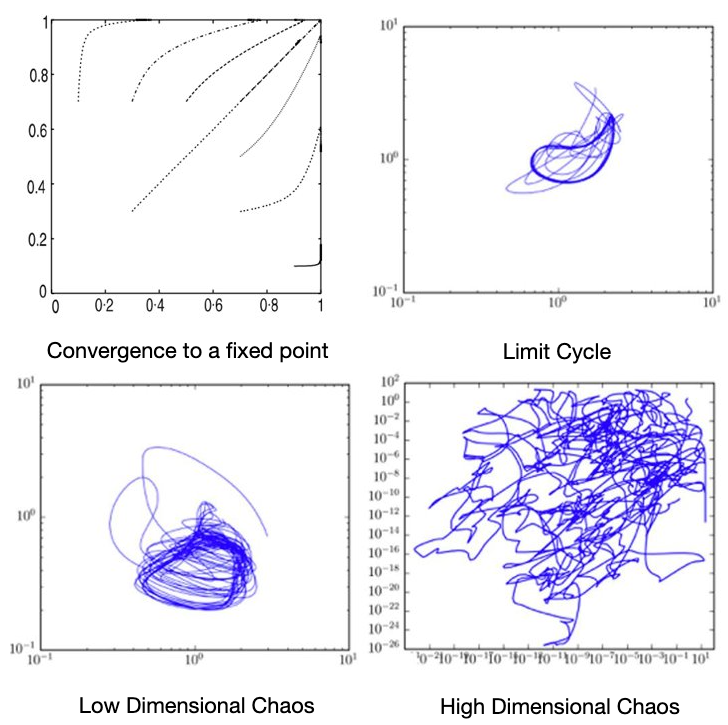
\includegraphics[width = \linewidth]{Figures/DynamicalBehaviours.png}
    \caption{Different types of dynamical behaviour
       displayed
        by learning agents. Here the $x$-axis (resp.~$y$-axis) is the probability with which agent 1 (resp.~agent 2) chooses a given action. (Top Left) Figure drawn from \cite{Tuyls2006AnGames}.
        Convergence
        to a unique fixed point at the point (1, 1). (Top Right) Limit Cycle, the trajectories converge to cyclic behaviour (Bottom)
        Chaotic behaviour, here small deviations in the initial conditions can grow
        exponentially. (Top Right) and (Bottom) drawn from \cite{Sanders2018}.}
\end{figure}

\subsection{Dynamics of Q-Learning}

The behaviour of a system may be studied given a model of its
dynamics. It is through this process that a wide array of physical
systems, from harmonic pendulums to geophysical fluids, can be
understood. A growing body of research aims to understand multi-agent
reinforcement learning through the lens of its dynamics. In this
light, \cite{Tuyls2006AnGames} presents of derivation of a continuous-time dynamical system describing how agents following a Q-Learning
approach adjust the probabilities of choosing actions as they
iteratively play a game. 

The games we consider are \textit{normal form games}. These consist of: a finite set of players, with individual strategy spaces $\mathcal{A}$ (though we assume that all players share the same strategy space) and payoff functions for each player. The agents choose an action from their strategy space and receive a reward from their payoff matrix dependent on the actions of all players. The payoffs remain unchanged across iterations. Examples of these normal form games include the popular Prisoner's Dilemma or Matching Pennies games \cite{Tuyls2006AnGames}.

The Q-Learning approach considered requires
an agent to choose an action $i$ at step $k+1$ with probability

\begin{equation}
    x_i(k) = \frac{e^{\tau Q_i(k)}}{\sum_j e^{\tau Q_j(k)}}
\end{equation}
%
where $\tau \in [0, \infty)$ is the \textit{intensity of choice} as described at the end of this section and $Q_i$ denotes the \textit{Q-value} of an action $i$, which is to be updated at each step according to
%
\begin{equation}
\label{eqn::Qupdate}
    Q_i(k+1) = (1 - \alpha) Q_i(k) + \alpha (r + \gamma \max_j Q_j(k))
\end{equation}
%
where $\alpha \in [0, 1]$ is the \textit{step length} parameter described below, $r$ is the immediate reward received, and $\gamma \in [0, 1]$ is the discount factor.

Through their analysis, Tuyls et al. were able to
arrive at the following dynamical model of multi-agent Q-Learning
%
\begin{subequations}
\label{eqn::EOM}
    \begin{equation}
        \frac{\dot{x}_i(t)}{x_i(t)} = \alpha \tau (\sum_{j} a_{ij} y_j - \sum_{i j} x_i a_{ij} y_j)
        + \alpha \sum_j x_j ln(\frac{x_j}{x_i}) 
    \end{equation}
    \begin{equation}
        \frac{\dot{y}_i(t)}{y_i(t)} = \alpha \tau (\sum_{j} b_{ij} x_j - \sum_{i j} y_i b_{ij} x_j)
        + \alpha \sum_j y_j ln(\frac{y_j}{y_i}).
    \end{equation}
\end{subequations}

Here,
agent 1 (resp.~agent 2) takes action $i$ with probability
$x_i$ (resp.~$y_j$).
When these actions are taken, the agents
receive payoff $a_{ij}$ and $b_{ji}$ respectively. With these equations, it is possible to
predict the expected behaviour of Q-Learning agents which they go on to empirically verify.

It is clear from (\ref{eqn::EOM}) that the long-term strategy
selection of these agents is determined by the parameters $\alpha,
\tau$ and the payoffs $a_{ij}, b_{ij}$. In light of this, this
contributions aims to address the question presented in the
introduction: how do these parameters influence the types of behaviours
seen during learning on an iterated game? Specifically, the parameters
we will consider are:
%
\begin{enumerate}
    \item $\alpha \in [0, 1]$: the \textit{step length}. Low values of $\alpha$ denote smaller
    updates. Heuristically, we can consider this to be the memory of the agent: lower $\alpha$
    denotes longer memory.
    
    \item $\tau \in [0, \infty)$: the \textit{intensity of choice}, as
      termed by Sanders et al.  \cite{Sanders2018}. This is sometimes
      written as $\beta$ in the literature \cite{Sutton2018}.  $\tau =
      0$ results in all actions being selected with equal probability,
      regardless of their Q-value, whilst $\tau \rightarrow \infty$
      results in the action with the highest Q-value chosen at every
      step. This may be seen as the \textit{exploration-exploitation
        parameter}. For greater details into these parameters, the
      interested reader should consult \cite{Sutton2018}.
    
    \item $\Gamma \in [-1, p-1]$: the \textit{payoff
      correlation}. Since there are an infinite number of realisations
      of the payoffs $a_{ij}, b_{ij}$, we instead analyse the
      behaviour for the average payoff case. To do this, we assume
      that the payoff matrices are drawn from a multi-variate Gaussian
      with mean zero and covariance matrix parameterised by
      $\Gamma$. We then average over this Gaussian. $\Gamma = -1$
      indicates a zero sum game, in which the sum of payoffs for a
      given action across all agents is 0, resulting in a purely
      competitive game. $\Gamma = p-1$ gives a purely cooperative game
      in which all agents share the same payoffs. The manner in which
      a game is generated from the choice of $\Gamma$ is described in
      (\ref{eqn::Payoffs}) below and follows the same procedure as
      outlined in \cite{Sanders2018}.
\end{enumerate}

%%%%%%%%%%%%%%%%%%%%%%%%%%%%%%%%%%%%%%%%%%%%%%%%%%%%%%%%%%%%%%%%%%%%%%%%

\section{Stability Analysis of Q-Learning} \label{sec::Theory}

In this section we aim to determine how the choice of parameters
$\alpha$ and $\tau$, alongside the choice of payoff matrix, affect the
stability of the dynamics of Q-learning. However, as the values in the
payoff matrix can take any real number, there is an infinite number
of possible realisations of games. Of course, it would not be possible
to analyse every possible game, we instead follow the procedure
outlined in \cite{Coolen2005} and \cite{Galla2013} to average over
these realisations and, instead, analyse the \textit{effective
  dynamics}, the dynamics averaged over all realisations of payoff
matrices. Then, we perform a linear stability analysis around
equilibrium points to determine the conditions under which a fixed
point is stable. As this process is rather involved, we focus on the main steps in this paper, and refer to the Supplementary Material for the technical details. Sections from the Supplementary Material are denoted with the prefix S.

\subsection{Rescaling of Variables}


Our first point of call is to extend the dynamics of Tuyls et al.~in
(\ref{eqn::EOM}a) and (\ref{eqn::EOM}b) to a general $p$-player
game. This yields the dynamics (\ref{eqn::pEOM}). Here, player $\mu$
chooses action $i_{\mu}$ from its strategy space $\mathcal{A}$ at time
$t$ with probability $\xmu{i}{\mu}$ and receives a reward
$\payoff{i}{\mu}$ from its payoff matrix $P^\mu$ depending on its own
action and the actions of all other agents $i_{-\mu}$, where $i_{-\mu}$ denotes the set $\{ i_\kappa : \kappa \in \{1, 2,
\ldots , p\} \setminus \{\mu\} \}$ and $-i_{\mu}$ denotes the set
$\mathcal{A} \setminus {i_\mu}$.
%
\begin{eqnarray}
%\begin{split}
    \frac{\dot{\xmu{i}{\mu}}}{\xmu{i}{\mu}} \! \! \! \! \! \! & = \! \! \! \! \! \! & \alpha \tau \left( \sum_{i_{-\mu}} \payoff{i}{\mu} \prod_{\kappa \neq \mu} \xmu{i}{\kappa} -  \sum_{i_\mu i_{-\mu}} \xmu{i}{\mu} \payoff{i}{\mu} \prod_{\kappa \neq \mu} \xmu{i}{\kappa} \right) \nonumber \\
    & & + \alpha \sum_{j_\mu \in -i_\mu} \xmu{j}{\mu} ln \frac{\xmu{j}{\mu}}{\xmu{i}{\mu}}     \label{eqn::pEOM}
%\end{split}
\end{eqnarray}

We now scale the system so that the probabilities sum to $N$. The
reason for this scaling is that, as the number of agents $p$ and
number of actions $N$ increases, the expected payoffs that agent
$\xmu{i}{\mu}$ receives all converge to the same value across its action
space. Therefore, the system must be scaled to ensure appreciable
differences across actions, so that the agent can choose its actions
appropriately (see the discussion in \cite{Sanders2018} or
Sec. S2.2 for further details). Accordingly we choose
scaled variables (denoted with a tilde or hat) as
%
\begin{eqnarray*}
%    \begin{split}
        \payoff{i}{\mu} & = & \tpayoff{i}{\mu} \sqrt{N^{p-1}}\\
        \xmu{i}{\mu} & = & \frac{\txmu{i}{\mu}}{N} \\
        \talpha & = & \frac{\alpha}{N}, \: 
        \ttau  =  N^{-(p-1)/2} \tau, \:
        \htau  =  N^{-p/2} \tau.
%    \end{split}
\end{eqnarray*}

The substitution in (\ref{eqn::pEOM}) yields the scaled equation
%
\begin{eqnarray}
%\begin{split}
    \frac{\dtxmu{i}{\mu}}{\txmu{i}{\mu}} & = & \alpha \ttau \left ( \sum_{i_{-\mu}} \tpayoff{i}{\mu} \prod_{\kappa \neq \mu} \txmu{i}{\kappa} \right ) \nonumber \\ & &  - \alpha \htau \left ( \frac{1}{\sqrt{N}} \sum_{i_\mu i_{-\mu}} \txmu{i}{\mu} \tpayoff{i}{\mu} \prod_{\kappa \neq \mu} \txmu{i}{\kappa} \right ) \nonumber  \\  & & + \talpha \sum_{j_\mu \in -i_\mu} \txmu{j}{\mu} ln \frac{\txmu{j}{\mu}}{\txmu{i}{\mu}}    \label{eqn::scaledEOM}
%\end{split}
\end{eqnarray}

Note that the scaled probabilities now satisfy the constraint
$\sum_{i_\mu} \txmu{i}{\mu} = N$. For the remainder of this derivation
we concern ourselves only with the scaled system so we drop the tilde
notation on $P$ and $x$.

As mentioned, we now
%wish to
generalise these dynamics to account for all the possible realisations
of the payoff matrix. To do this, we assert that the payoff elements
(after scaling) are generated by a multi-variate Gaussian distribution
with mean zero and covariance given as
%
\begin{equation}
\label{eqn::Payoffs}
%    \begin{split}
        \mathbb{E}\left [ \payoff{i}{\mu} \payoff{i}{\nu} \right] = \begin{cases}
        \frac{1}{N^{p-1}} &  \text{ if } \nu = \mu \\
        \frac{\Gamma}{(p-1) N^{p-1}} & \text{ otherwise. }
        \end{cases}
%    \end{split}
\end{equation}

The motivation for choosing that the payoffs is generated by a
Gaussian is that it allows for the use of Gaussian identities when
determining the average.

\subsection{The Effective Dynamics}

We then use a generating functional approach as outlined in
\cite{Mezard1986} to average the dynamics over this multi-variate
Gaussian. The generating functional is a method derived from
statistical mechanics which allows for expectations to be taken over
equations of motion and, in particular, allows for the analysis of
systems with `quenched disorder': these are
variables which are random but held fixed in time as the system
evolves (in our case these variables are the payoff elements). The
generating functional for the equation of motion (\ref{eqn::scaledEOM}) is given as \cite{Mezard1986}

{\small
\begin{equation}
\label{eqn::separatePayoffs}
	\begin{split}
	Z(\Vec{\psi}) = \int D[\Vec{x}, \Vec{\hat{x}}] exp( i \sum_{i, \mu} \int dt [ \hxmu{i} (\frac{\dxmu{i}}{\xmu{i}{\mu}} - \talpha \rho_i^\mu (t) - h_i^\mu (t))]) \times \\ exp(-i \alpha \ttau \sum_{\mu} \sum_{i_\mu, i_{-\mu}} \int dt [\hxmu{i} \payoff{i}{\mu} \prod_{\kappa \neq \mu} \xmu{i}{\kappa} )])) 
    \times \\ exp(-i \alpha \ttau \sum_{\mu} \sum_{j_\mu, i_\mu, i_{-\mu}} \int dt [\hxmu{j}  \xmu{i}{\mu} \payoff{i}{\mu} \prod_{\kappa \neq \mu} \xmu{i}{\kappa}])) 
	\times \\ exp(i \sum_{i, \mu}
	\int dt[\xmu{i} \psi^\mu_i(t)]),
\end{split}
\end{equation}
}
where the `generating fields' \cite{Coolen2005} $\Vec{\psi_i(t)}$ and
$\Vec{\phi_i(t)}$ will be set to zero at the end of the
calculation.

The last two exponentials contain the payoffs of the game. These are randomly generated using a multi-variate gaussian and then held fixed for the rest of the game. As such these comprise the aforementioned `quenched disorder'. We will average over this quenched disorder (and therefore average over all possible realisations of payoff matrices) using the mean and covariance expressions given in (\ref{eqn::Payoffs}). We define $Q$ to be the product of the second and third exponentials in (\ref{eqn::separatePayoffs}) 
%
\begin{equation}
\begin{split}
        \mathbb{E}[Q] = exp(- \frac{\alpha^2 \ttau ^2}{2} N \sum_{\mu} \Big [ \int dt dt' L^\mu(t, t') \prod_{\kappa \neq \mu} C^\kappa (t, t') + \\ \Gamma \sum_{\nu \neq \mu} K^\mu (t, t') K^\nu (t, t') \prod_{\kappa \not\in \{\mu, \nu\}} C^\kappa (t, t') \Big ] ) \times \\
        exp(- \frac{\alpha^2 \htau ^2}{2} N \sum_{\mu} \Big [ \int dt dt' L^\mu(t, t') C^\mu (t, t') \prod_{\kappa \neq \mu} C^\kappa (t, t') + \\ \Gamma \sum_{\nu \neq \mu} A^{\mu \nu} (t, t') C^\nu (t, t') C^\mu (t, t') \prod_{\kappa \not\in \{\mu, \nu\}} C^\kappa (t, t') \Big ] )
\end{split}
\end{equation}
%
in which
%
\begin{eqnarray*}
\label{eqn::correlations}
%    \begin{split}
        C^\mu (t, t') &  := & N^{-1} \sum_i \xmu{i}{\mu} \xmudash{i}{\mu} \\
        L^\mu (t, t') & :=  & N^{-1} \sum_i \hxmu{i} \hxmudash{i} \\
        K^\mu (t, t') & :=  & N^{-1} \sum_i \xmu{i}{\mu} \hxmudash{i} \\
        A^{\mu, \nu} (t, t') & := &  N^{-1} \sum_i \hxmu{i} \hxnudash{i}.
%    \end{split}
\end{eqnarray*}

By taking this average (Sec. S2.3), we obtain the \textit{effective dynamics}
%
\begin{eqnarray}
    \label{eqn::EffectiveDynamics}
%    \begin{split}
            \frac{1}{x} \frac{d}{dt} x(t) & = & \alpha^2 \ttau^2 \Gamma \int dt' \left [G(t, t')C^{p - 2}(t, t') x(t') \right ] \nonumber \\ && + \sqrt{2} \alpha \ttau \eta_1(t) + \sqrt{2} \alpha \htau \eta_0(t) + \talpha \rho(t), 
%    \end{split}
\end{eqnarray}
%
in which we have assumed that all players' actions are independent and drawn from the same initial distribution (i.i.d)
and therefore dropped the distinction between players and strategy components. The terms $G, C, \eta_1, \eta_0$ are correlation functions, generated when averaging the Gaussian. These are given as 
%
\begin{eqnarray*}
%    \begin{split}
        C(t, t') & = & \mathbb{E}[x(t) x(t')] \\
        \mathbb{E}[\eta_1(t)] & = & 1, \text{ \space } \mathbb{E}[\eta_1(t) \eta_1(t')]  =  C^{p-1}(t, t') \\
        \mathbb{E}[\eta_0(t)] & = & 1, \text{ \space } \mathbb{E}[\eta_0(t) \eta_0(t')] = C^{p}(t, t') \\
        G(t, t') & = & \mathbb{E}\left [ \frac{\delta x(t)}{ \delta \eta_1(t')} \right].
%    \end{split}
\end{eqnarray*}

It is important to note the effect of the former assumption (that all
actions of all agents are i.i.d) is substantial. With this assumption,
we identify the coupled term $A^{\mu, \nu} (t, t')$ in
(\ref{eqn::correlations}) with the uncoupled term $L^\mu (t, t')$
(since there is no distinction between the actions of agents $\mu$ and
$\nu$). This is a strong assumption which removes the interdependency
between agents in the analysis and is required to ensure that (\ref{eqn::EffectiveDynamics}) yields real-valued action probabilities. However, as shown by the experimental
evaluation, it does not produce a strong discrepancy in describing the
qualitative effect on stability caused by the parameters $\alpha$, $\Gamma$, and $\tau$.

\subsection{Linear Stability Analysis}

We first find a fixed point $\xfixed$ of (\ref{eqn::EffectiveDynamics}) by letting $\dot{x}(t)= 0$. This yields the expression 
%
%\small{
\begin{equation}
%    \begin{split}
    0  = \xfixed [ \alpha^2 \ttau^2 \Gamma \xfixed q^{p-2} \chi + \sqrt{2} \alpha \ttau q^{(p-1)/2}z + \sqrt{2} \alpha \htau q^{p/2} z^{p/p-1} + \talpha \rho]
    \label{eqn::fixed_point}
%    \end{split}
\end{equation}
%}
%
where $\chi = \int dt' G(t - t')$, $\eta_0(t) = q^{(p-1)/2}z$, $z$ is
drawn from a Gaussian of zero mean and unit variance. By using (\ref{eqn::fixed_point}) we can
%his gives us an expression for
calculate $\xfixed$. We disregard the choice $\xfixed = 0$, since we
assume that no action will be chosen with exactly zero probability, an
intuitive assumption which is also considered in \cite{Sanders2018}
and \cite{Coolen2005}. The expression inside the squared bracket
admits a positive solution only in the region $\Gamma \in [-1, 0]$,
whilst for positive $\Gamma \leq p-1$, the nature of solutions may
not be guaranteed. Therefore, we restrict our analysis to the region
$[-1, 0]$.

We now analyse the stability of the system (\ref{eqn::EffectiveDynamics}) in a neighbourhood around
this fixed point. This follows a similar procedure as in \cite{Opper1992}, in
which the fixed point dynamics are proposed to be perturbed by a
disturbance $\xi(t)$ which is drawn from a Gaussian of zero mean and
unit variance. The disturbance causes the values of $x(t)$ and
$\eta_0(t), \eta_1(t)$ to deviate from their fixed point position
$\xfixed, \ezerof, \eonef$ by an amount $\xpert, \ezeropert,
\eonepert$.  If we consider only the terms which are linear in these
perturbations, we arrive at 
%
\begin{eqnarray}
%    \begin{split}
\frac{d}{dt} \xpert & = & (\xfixed + \xpert) [ \alpha^2 \ttau^2 \Gamma \xfixed \int dt' [ G(t, t')C^{p - 2}(t, t') ] \nonumber \\
  & & + \sqrt{2} \alpha \ttau \eonef + \sqrt{2} \alpha \htau \ezerof + \talpha \rho] \nonumber \\
& &  + \xfixed [\alpha^2 \ttau^2 \Gamma \int dt' [ G(t, t')C^{p - 2}(t, t') \xpertdash ] \nonumber \\
  & & + \sqrt{2} \alpha \ttau \eonepert + \sqrt{2} \alpha \htau \ezeropert + \xi(t)].
\label{eqn::Linearised}
%    \end{split}
\end{eqnarray}

We then examine the
long-term behaviour of the perturbation $\xpert$. by taking
the Fourier transform of (\ref{eqn::Linearised}) and analysing its
behaviour at $\omega = 0$. After some manipulation (Sec. S4), this gives
%
\begin{equation}
%\begin{split}
        \mathbb{E}[|\mathcal{X}(\omega = 0)|^2] = \frac{1}{\left[ (-\alpha^2 \ttau^2 \Gamma q^{p-2} \chi)^2 - 2 (\alpha \ttau + \alpha \htau)^2 (p-1)q^{p-2}\right]} 
%\end{split}
\end{equation}

As the left hand side of this equation must be greater than zero, we arrive at the condition that, at a fixed point, the long term perturbations must satisfy
%
\begin{equation}
    \label{eqn::Final}
    0 \leq \left [(\alpha^2 \ttau^2 \Gamma q^{p-2} \chi)^{2} - 2 (\alpha \ttau + \alpha \htau)^2 (p-1)q^{p-2} \right ]
\end{equation}

It should be noted that, to arrive at this result, we have had to take the assumption that p is large enough so that $p/p-1 \approx 1$ so that the fractional power on $z$ in (\ref{eqn::fixed_point}) is reduced to $1$. As $z$ can take any value, including negative values, this again ensures that the expression for $\xfixed$ remains real valued.

\subsection{Discussion}



The fixed point condition (\ref{eqn::Final}) yields a number of testable implications, of which we subsequently test the validity. These implications are as follows.

\begin{enumerate}
    \item A trivial result is that the game is everywhere convergent (i.e. regardless of the choice of $\Gamma, N, p$) for the cases of $\alpha$ = 0 and/or $\tau$ = 0.  We see that choosing these values would result in the right hand side of (\ref{eqn::Final}) yielding a value of zero which falls within the stable region.
    \item Convergence is rare. This is seen by the fact that the analytic result overestimates the region of instability. In fact, for all allowed choices of $\Gamma, \alpha, \tau$, the right hand side of (\ref{eqn::Final}) is negative, which violates the stability criterion. This implies that games, in general, will not converge.
    \item The likelihood of convergence decreases with increasing $\alpha$ and $\tau$, regardless of the choice of $N, p$. We can see this since the right hand side of (\ref{eqn::Final}) tends further away from zero (i.e. further from the region of stability).
    \item The choice of $\Gamma$ does not affect the stability of the game in the negatively-correlated regime. Therefore, the only dependent factors are $\alpha, \tau, N, p$. This is more easily interpreted from the heatmaps in Figure \ref{fig:theory}.
    \item The likelihood of convergence decreases as $p$ increases. We see this by noticing the weighting that the $(p-1)$ in the second term of (\ref{eqn::Final}) places. As $p$ increases, this term drives the system further from the stability boundary.

\end{enumerate}

We illustrate these implications in Figure \ref{fig:theory} which plots the value obtained by the right hand side of (\ref{eqn::Final}). In order to determine these values, we first had to solve (\ref{eqn::fixed_point}) for $q$ and $\chi$. We determine the $\xfixed$ which solves the expression inside the square brackets of (\ref{eqn::fixed_point}) using a Newton-Raphson root-finding approach and use the following expressions for $q, \chi$ to determine their value. 
%
\begin{eqnarray*}
%    \begin{split}
        1 & = & \frac{1}{\sqrt{2 \pi}} \int_{-\infty}^{\infty} \xfixed(z) exp(-\frac{z^2}{2}) dz \\ 
        q & = & \frac{1}{\sqrt{2 \pi}} \int_{-\infty}^{\infty} \xfixed(z)^2 exp(-\frac{z^2}{2}) dz \\ 
        \chi & = & \frac{1}{q^{n/2}}\frac{1}{\sqrt{2 \pi}} \int_{-\infty}^{\infty} \frac{\partial \xfixed (z)}{\partial z} exp(-\frac{z^2}{2}) dz
%    \end{split}
\end{eqnarray*}

It should note that this method of finding $\xfixed$ yields only an approximate value and so the $q, \chi$ which are found are estimates of their true value. 

We consider each of the implications (2)-(5) from the Sec. \ref{sec::Theory}
in turn, choosing to forego illustrating (1) as it can be seen immediately
from (\ref{eqn::Final}). $\tau$ is held fixed
at $0.05$ and vary $\Gamma$ in
the range $[-1, 0]$, $\alpha$ in the range $[0.01, 0.05]$.

\paragraph{Implication 2:} By looking at the values of the heatmap, we see that, for all choices
of the parameters
(\ref{eqn::Final}) evaluates to a negative value, which signals
instability. As such, the analysis over-estimates the region of
instability. We believe that this is due to the
%heavy
assumptions made during the derivation of the analytic result, the
strongest of which was to drop the discrepancy between players and
actions, treating each action of each player to be independent and
identically distributed. However, even within the error that this
assumption generates, it is still clear (and is verified
experimentally) that (\ref{eqn::Final}) predicts convergence in Q-Learning to be rare. Indeed as the
value of $N$ increases, the stability boundary determined by
experiment (Figure \ref{fig:NumericalExperiments}) tends towards
$\alpha = 0, \tau = 0$.

Similarly, as the value of $N$ increases, the values in the heatmap
(seen on the right of the map) reduce. This is due to the assumption
made in the derivation of the analytic result that $N \rightarrow
\infty$. As the value of N increases, the discrepancy between the true
behaviour of the system and analytic result decreases. This does,
however, give rise to a limitation of the result - namely that the
effect of the number of actions $N$ cannot be accurately inferred from
 (\ref{eqn::Final}). However, it should still be noted that, even
with the increase of $N$, the values in parameter space remain negative
and still, accurately, predict instability. We go on to verify that
the effect of $p, \alpha, \Gamma$ and $\tau$ are accurately captured
by (\ref{eqn::Final}).

We interpret (\ref{eqn::Final}), for given parameters, by determining
how close the right hand side is to the stability boundary (i.e., how
close the value is to zero). A choice of parameters which evaluates
close to the stability boundary has a higher chance (by the analytic
error) of being convergent than one which lies further from the
boundary. Therefore, the heat-maps in Figure \ref{fig:theory} should
be considered to show the probability of convergence for a choice of
$(\alpha, \Gamma)$. Lighter regions denote a higher probability of
convergence whereas darker regions are those whose values are further
from zero and therefore show a lower probability of convergence.

\paragraph{Implication 3} can be visualised by noticing that the likelihood of convergence decreases (the heatmap becomes darker) as $\alpha$ increases, and similarly for $\tau$. This occurs independent of the choice of $N$ or $p$. 

\paragraph{Implication 4} can similarly be inferred by the trend of convergence, which occurs only in varying $\alpha$. The choice of $\Gamma$
makes almost no difference in the evaluation of (\ref{eqn::Final}). We
anticipate that this is due to the restriction of $\Gamma$ to be in
the range $[-1, 0]$. In this range, the scaling effect of $\Gamma^2$
is dominated by the $\alpha^4$ and $\tau^4$ terms which appear in
(\ref{eqn::Final}).

\begin{figure}[t]
    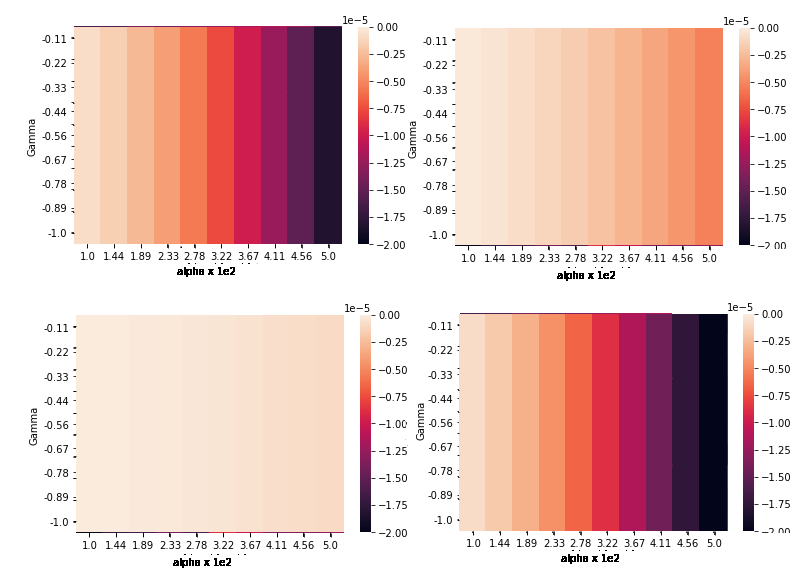
\includegraphics[width = 1.2 \linewidth, center]{Figures/Theory.png}
    \caption{Evaluation of (\ref{eqn::Final}) over a range of $\alpha$ and $\Gamma$ values. Ligher regions indicate where (\ref{eqn::Final}) is close to zero (i.e. close to the stability boundary) whilst darker regions are further away. We vary $\alpha$ in the range $[0.01, 0.05]$ and $\Gamma$ in the range $[-1, 0]$. $\tau = 0.05$. (Top Left) $p = 2, N = 2$, (Top Right) $p = 2, N = 5$, (Bottom Left) $p = 2, N = 20$, (Bottom Right) $p=3, N = 2$.}
    \label{fig:theory}
\end{figure}

\begin{figure}[t]
    \centering
    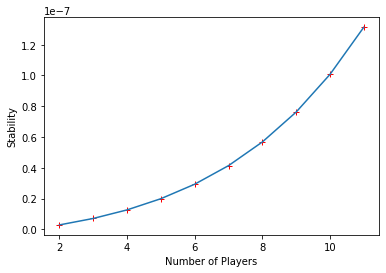
\includegraphics[width = .75\linewidth]{Figures/pVariance.png}
    \caption{Evaluation of (\ref{eqn::Final}) for varying numbers of players $p$. Here, $\alpha$ is fixed at $0.02$, $\tau = 0.05$, $N = 2$ and $\Gamma = -1$. $p$ is varied from 2 to 12. We see that the value obtained by (\ref{eqn::Final}) tends away from zero monotonically.}
    \label{fig:pvariation}
\end{figure}

\paragraph{Implication 5}, finally, is considered in Figure \ref{fig:pvariation}. In this we keep all parameters, except for $p$, fixed and evaluate the right hand side of (\ref{eqn::Final}) for varying $p$, taking the absolute value for convenience. We see that the trend is to tend away from the stability boundary, indicating that as the number of players in the system increases, so too does the region of instability.


%%%%%%%%%%%%%%%%%%%%%%%%%%%%%%%%%%%%%%%%%%%%%%%%%%%%%%%%%%%%%%%%%%%%%%%%

\section{Experimental Evaluation} \label{sec:exev}

In this section, we describe and discuss the numerical experiments we use to verify the implications described in the discussion of Sec. \ref{sec::Theory}. We first describe how these experiments were conducted and then, having presented the results in Figures \ref{fig:NumericalExperiments} and \ref{fig:pVarianceExpt}, we discuss the correlation with the theory.

\subsection{Construction of Numerical Experiments}

To verify experimentally the theoretical results, and to examine the underlying structure of stability and chaos in
Multi-Agent Q-Learning, we perform a series of numerical experiments by varying the parameters $\Gamma$ and
$\alpha$ whilst keeping $\tau$ fixed. The aim is to determine the regions in which games learnt using Q-Learning converge to an equilibrium. The results of these experiments are shown in Figure \ref{fig:NumericalExperiments}, with parameters chosen to match those in the analytic assessment (Figure \ref{fig:theory}).

To generate the numerical simulations in Figure~\ref{fig:NumericalExperiments} we used the
following procedure.
\begin{enumerate}
   \item Fix the parameters $\tau, \gamma$. The former is held at 0.05 and the latter at 0.1.
   \item Initialise values of $\Gamma, \alpha$ (or $\tau$ appropriately). These will be swept over in the experiment.
\item Generate 15 payoff matrices by sampling from a multi-variate Gaussian 
(variables are the payoff elements) with mean zero and covariance parameterised by $\Gamma$.
\item For each of these payoff matrices, initialise a set of agents with random initial conditions (i.e., random action probabilities).
\item Allow both sets of agents to learn over a maximum of $1.5 \times 10^4$ iterations.
\item Keep track of the action probabilities over a window of 500 iterations. At the end of each window, determine the percentage difference between the maximum and minimum values of each strategy component
\item If the difference is less than 1\% consider the game converged. Otherwise continue to the next window.
\item If the game reaches $1.5 \times 10^4$ iterations without satisfying the relative distance criterion, consider it to be non-convergent. Determine the fraction of these 15 games which have converged.

\end{enumerate}
   
We see in Figure \ref{fig:NumericalExperiments} that the stability of the system is highly dependent on
the value of $\alpha$ and $\tau$ but not on $\Gamma$.
   
\begin{figure}[t]
    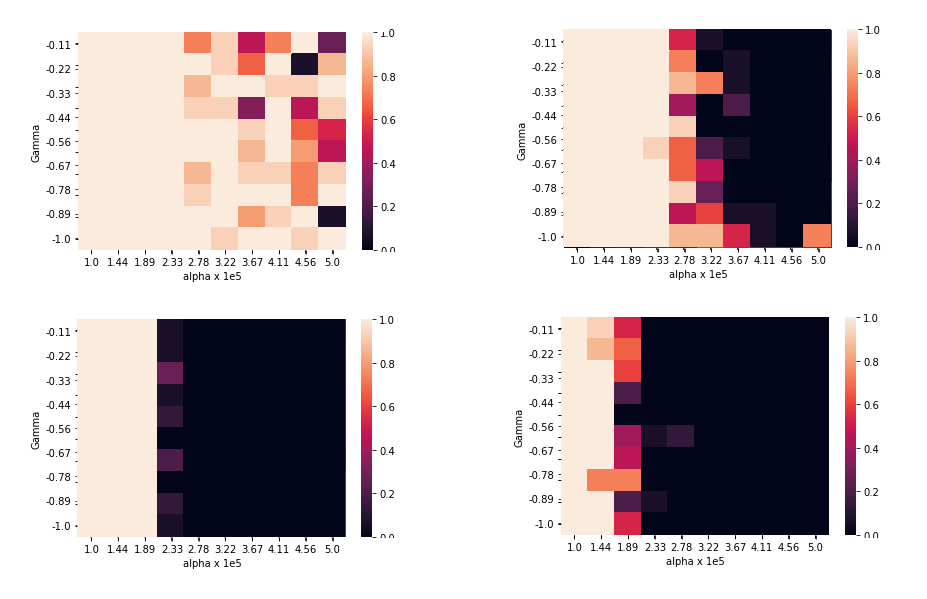
\includegraphics[width = 1.2 \linewidth, center]{Figures/Experiments.png}
    \caption{Results of numerical experiments in which $\alpha$ is varied. The heatmaps show the fraction of games which converge to an equilibrium. Lighter values show higher convergence. Each experiment is run with $\tau = 0.05$. (Top Left) $p = 2, N = 2$, (Top Right) $p = 2, N = 5$, (Bottom Left) $p = 2, N = 20$, (Bottom Right) $p=3, N = 2$.}
    \label{fig:NumericalExperiments}
\end{figure}

\begin{figure}[t]
    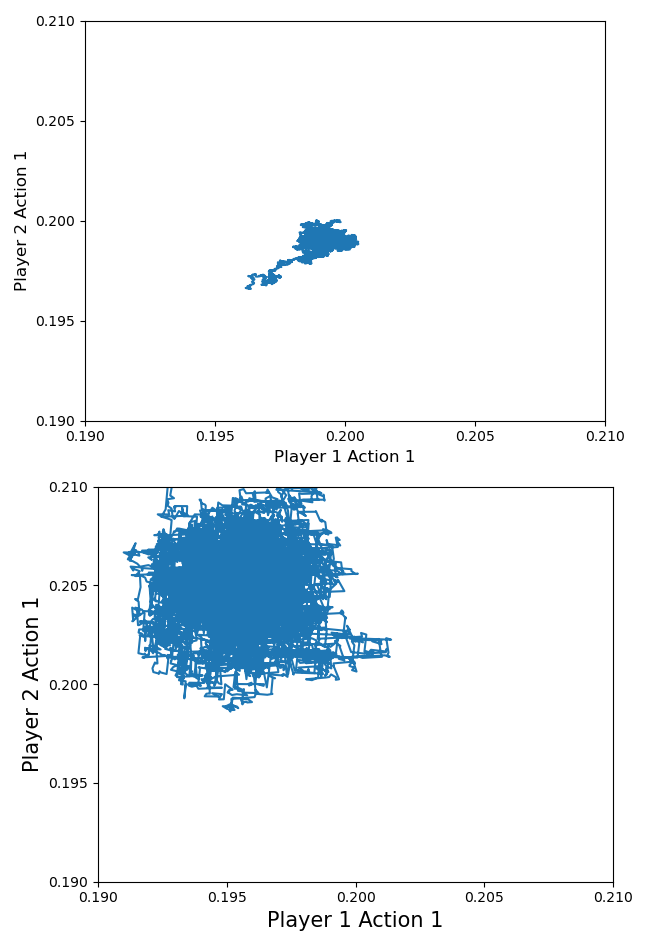
\includegraphics[width =  \linewidth, center]{Figures/alphavar5e2.png}
    \caption{The trajectories of action probabilities for 2 players with 5 actions trained on a game of $\Gamma = -0.5$ and $\tau = 0.05$. (Left) $\alpha = 0.01$, (Right) $\alpha = 0.05$.}
    \label{fig:AlphaVariation}
\end{figure}

In Figure \ref{fig:AlphaVariation}, we explicitly plot the trajectories taken by the action probabilities as two agents are trained on a game of $\Gamma = -0.5$. In the left figure, we choose $\alpha = 0.01$ whilst in the right we choose $\alpha = 0.05$. We note that the typical behaviour of the system is that the system first moves towards a fixed point and then varies in a pseudo-random manner within a vicinity of the fixed point. Critically though, the amount of variation in the case $\alpha = 0.05$ is greater than that of $\alpha = 0.01$. 

\begin{figure}[t]
    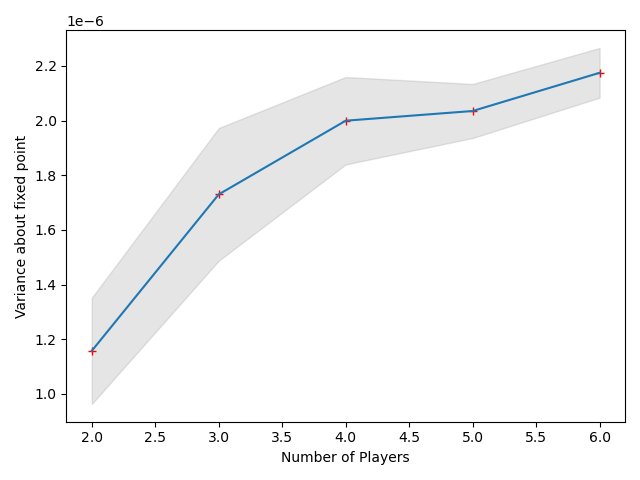
\includegraphics[width = .75\linewidth, center]{Figures/pVarianceExpt.png}
    \caption{Variation $V(t)$ about a fixed point as $p$ ranges from 2 - 6. $N = 2$, $\alpha = 0.02$, $\tau = 0.05$, $\Gamma = [-1, 0]$. The experiment is conducted for 10 choices of $\Gamma$ and the mean (line) is plotted alongside the standard deviation (shaded region).}
    \label{fig:pVarianceExpt}
\end{figure}

Finally, Figure \ref{fig:pVarianceExpt} plot the degree variation about the fixed point displayed as the number of players $p$ increases. The variation is determined by first allowing the game to iterate for 5000 steps, so that it can be assumed to have reached the vicinity of the fixed point. Then, the action probabilities are recorded for a further 5000 iterations. At the end of this second period, the variance of the actions are calculated as
%
\begin{equation*}
    V(t) = \frac{1}{N} \sum_i \frac{1}{5000} \sum_t x_i(t)^2 - \left[\frac{1}{5000} \sum_t x_i(t) \right]^2 .
\end{equation*}

This gives a measure of the degree of variability about the fixed point and, therefore, gives some notion of the `degree of instability'. For example, the right hand plot of Figure \ref{fig:AlphaVariation} has a higher $V(t)$ than the left and so is considered to show a higher degree of instability. 

Due to computational restraints, which we discuss further in the discussion, we are only able to increase $p$ to a maximum value of 6 and must restrict also to $N = 2$. We maintain $\alpha = 0.02$ and $\tau = 0.05$ to match with the parameters used for Figure \ref{fig:pvariation}. Finally, in Figure \ref{fig:pVarianceExpt}, we are averaging over 10 choices of $\Gamma$ in the range $[-1, 0]$. 

\subsection{Discussion}
    
We note that the numerical experiments confirm the predictions
suggested by the analytic results in Figure
\ref{sec::Theory}. We notice that convergence occurs almost only for
low values of $\alpha$. This observation remains as we increase the
value of $N$. As noted, the analytic result over-estimates the region
of instability due to the assumptions of $N \rightarrow \infty$ and
$\frac{1}{p-1} << 2$ made during the derivation. Remaining
discrepancies are partially due to the aforementioned approximation in
the calculation of $q$, $\chi$ and the fact that the analytic result
considers a continuous time approximation of the expected behaviour of
Q-Learning. We expect that testing over a greater number of payoff
realisations and initial conditions will yield a more representative
assessment of the average behaviour of Q-Learning. However, running
these experiments is a computationally expensive procedure: for $p$
players and $N$ actions we require operations on $p$ matrices with
$N^{p}$ elements. As such, due to a reduced availability of
computational facilities, a large scale averaging was not possible.

However, due to the prevalence of non-convergent behaviour, shown by
the dark regions in Figure \ref{fig:NumericalExperiments} other than
at low values of $\alpha, \tau$, we conclude that implications (1),
(2) are verified. Indeed, implication (3) and (4) are also verified as
the proportion of games converged decrease monotonically with
$\alpha$, $\tau$, but there does not appear to be any discernible
dependence on $\Gamma$. Finally, we can conclude that implication 5 is
verified by comparing Figures \ref{fig:pvariation} and
\ref{fig:pVarianceExpt}. It is clear that the instability of the
system increases monotonically with $p$. A point to note is that
Figure \ref{fig:pVarianceExpt} shows a logarithmic dependence of the
instability on $p$, whilst Figure \ref{fig:pvariation} suggests that
the dependence should be exponential. Due to the limited range of $p$
that was used to generate Figure \ref{fig:pVarianceExpt}, it cannot
yet be concluded that the dependence on $p$ is logarithmic. However,
the key point is that, as $p$ increases, the unstable behaviour
increases, regardless of parameter choice, which is corroborated by
both theory and experiments. This phenomenon was referred to in
\cite{Sanders2018}
%by Sanders et. al
as `the prevalence of chaotic dynamics in games with many
players'.

A point which we wish to discuss here is the difference in the result
found w.r.t.~\cite{Sanders2018}, which considered the stability of
\textit{experience weighted attraction} (EWA). Namely, Sanders et
al.~found that convergence is seen for higher values of $\alpha$,
whereas lower values give rise to chaos, the opposite of what is found
here. The reason for this can be seen in the update equation of
Q-Learning (\ref{eqn::Qupdate}), whereby smaller values of $\alpha$
result in the agent placing a lower weight on the reward received at
each step. As such, lower values of $\alpha$ result in the agent
taking more conservative steps and yields a higher probability of
convergence. In contrast, the update for EWA does not discount the
reward received at all and, instead, only discounts the previous
knowledge of the Q-value based on higher choices of $\alpha$. In
essence, the difference is the fact that Q-Learning discounts new
information by a factor of $\alpha$, whilst EWA does not. Yet, the
difference in stability caused by this change is significant. This
highlights the importance of performing analyses such as the present
work; it allows for a method to analytically compare the difference
between learning algorithms and, for practitioners, ensure that the
appropriate algorithm is chosen for the parameters of their specific
task.


To summarise, we have shown that the analytic result
(\ref{eqn::Final}) provides a strong assessment for the effect that
$\alpha$, $\tau$, $\Gamma$ and $p$ have on the likelihood of
convergence of Q-Learning. We showed that, at least for negatively
correlated payoffs, the strength of correlation plays no role in
determining the stability of the system. Furthermore, though
(\ref{eqn::Final}) overestimates the region of instability, it
accurately conveys that convergence of Q-Learning is unlikely for
games with many players and actions. In fact, our experimental results
also verify that stability may only be guaranteed for the limiting
case of two-player, two-action games. Once either of these parameters increase, the region of instability increases rapidly.
%
Finally, we showed that the behaviour of the stability line differs
from that of EWA and suggest that this shows that a stability analysis
is an important mode of analysis for reinforcement learning algorithms
to ensure that parameters are being chosen appropriately to guarantee
the safe convergence of learning.

\section{Conclusion}

In this study, we made a first contribution towards the
characterisation of the behaviours of agents learning how to play
$p$-player, $N$-action games through Q-Learning. To this end, we
analysed the replicator model of Q-Learning derived in \cite{Tuyls2006AnGames}. Specifically, we searched for the regions in parameter space
where the dynamics are expected to converge to a stable equilibrium
and those where learning is unstable. This yielded a number of
important results. We showed that convergence to a unique fixed point is
found for low values of $\alpha$, the \textit{step length} of the
algorithm, and for negatively correlated payoff matrices, though the
strength of correlation $\Gamma$ does not influence stability. As
$\alpha$ increases, the likelihood of convergence decreases. The same
is true for the \textit{intensity of choice} parameter $\tau$. Our
analysis also shows that the likelihood of convergence decreases,
regardless of parameter choice as the number of players $p$ in the
system increases.

\paragraph{Future Work}
Our first aim is to verify the analytic results at a finer resolution
and by averaging over a greater number of payoff realisations. This
will give a greater insight into the boundary between convergent and
non-convergent behaviour and allow for practitioners to choose their
parameters in such a way that convergence to a (possibly unique) fixed
point can be expected. In addition we noted that one of the conclusions of
our study is that convergence to a unique fixed point is rare in
Q-Learning. In fact, complex behaviours (such as the existence of
multiple fixed points, limit cycles, and chaos) are more likely. We,
therefore, aim to characterise these complex behaviours in parameter
space both theoretically and numerically.

% The present work represents a first step towards considering the stability
% of multi-agent reinforcement learning and focuses on the limiting case
% of stateless normal-form games played by homogeneous agents.
As
research into the dynamics of RL algorithms
progresses, it would be prudent to apply this analysis to various
other algorithm. Algorithms whose dynamics are established, and are
therefore open to a stability analysis, include piecewise Q-Learning
and Cross Learning. This would provide a strong method by which to
compare and provide safety guarantees to different algorithms for a
particular use case.

%%%%%%%%%%%%%%%%%%%%%%%%%%%%%%%%%%%%%%%%%%%%%%%%%%%%%%%%%%%%%%%%%%%%%%%%

%%% The acknowledgments section is defined using the "acks" environment
%%% (rather than an unnumbered section). The use of this environment 
%%% ensures the proper identification of the section in the article 
%%% metadata as well as the consistent spelling of the heading.

\begin{acks}
If you wish to include any acknowledgments in your paper (e.g., to 
people or funding agencies), please do so using the `\texttt{acks}' 
environment. Note that the text of your acknowledgments will be omitted
if you compile your document with the `\texttt{anonymous}' option.
\end{acks}

%%%%%%%%%%%%%%%%%%%%%%%%%%%%%%%%%%%%%%%%%%%%%%%%%%%%%%%%%%%%%%%%%%%%%%%%

%%% The next two lines define, first, the bibliography style to be 
%%% applied, and, second, the bibliography file to be used.

\newpage

\bibliographystyle{ACM-Reference-Format} 
\bibliography{references}

%%%%%%%%%%%%%%%%%%%%%%%%%%%%%%%%%%%%%%%%%%%%%%%%%%%%%%%%%%%%%%%%%%%%%%%%

\end{document}

%%%%%%%%%%%%%%%%%%%%%%%%%%%%%%%%%%%%%%%%%%%%%%%%%%%%%%%%%%%%%%%%%%%%%%%%
